\documentclass[12pt,a4paper]{article}
\pagestyle{plain}
\usepackage{fullpage}
\usepackage[english]{babel}
\usepackage{enumerate}

%equations
\usepackage[fleqn]{amsmath}
\numberwithin{equation}{section}

%figures
\usepackage[dvips]{graphicx}
\graphicspath{{./images/}}
\numberwithin{figure}{section}

%excercises
\newcounter{Exercise}
\setcounter{Exercise}{1}
\usepackage[dvipsnames]{xcolor}
\usepackage{framed}
\definecolor{shadecolor}{gray}{0.9}
\usepackage{caption}

%tables
\numberwithin{table}{section}

%specials
\usepackage{textcomp} %special (greek) characters as text
%\usepackage{pstricks} %
%\usepackage{ifthen} %
%\usepackage{calc} %
%\usepackage{isotope}
\usepackage{hyperref}
\usepackage[bottom]{footmisc} %footnote below figure
\usepackage{footnpag}%number footnotes per page


%document details
\author{J. Kortland \\ translated and adapted by K. Schadenberg}
\date{}
\title{Sources of Cosmic Radiation}


\begin{document}
\maketitle

\section{Introduction}
Our planet, Earth, is constantly bombarded with particles from space: Cosmic Radiation. A large part of these particles are neutrinos and hydrogen nuclei (single protons), but there are also heavier particles headed for Earth.
In this module we will look at the energy of the particles hitting our atmosphere and what this tells us about the possible origins or sources of these particles.

\section{Energy}
There have been a large number of experiments trying to measure the different energy levels of cosmic radiation. The combined results of these experiments tell us that the energy of charged cosmic particles, such as single protons or heavier atomic nuclei, varies from less than 10$^9$ up to (or possible slightly above) 10$^{20}$~eV.\footnote{The abbreviation eV stands for electron volt, a measure of energy just like the Joule. For more information about this measure of energy read the module `Primary Particle - Energy'.}

With increasing energy the number of detected particles rapidly decreases, this can be seen in figure~\ref{fig:spectrum}.\footnote{Take a good look at the scaling and the units of both axes.} The origins of these particles are very diverse.

\begin{figure}\begin{center}
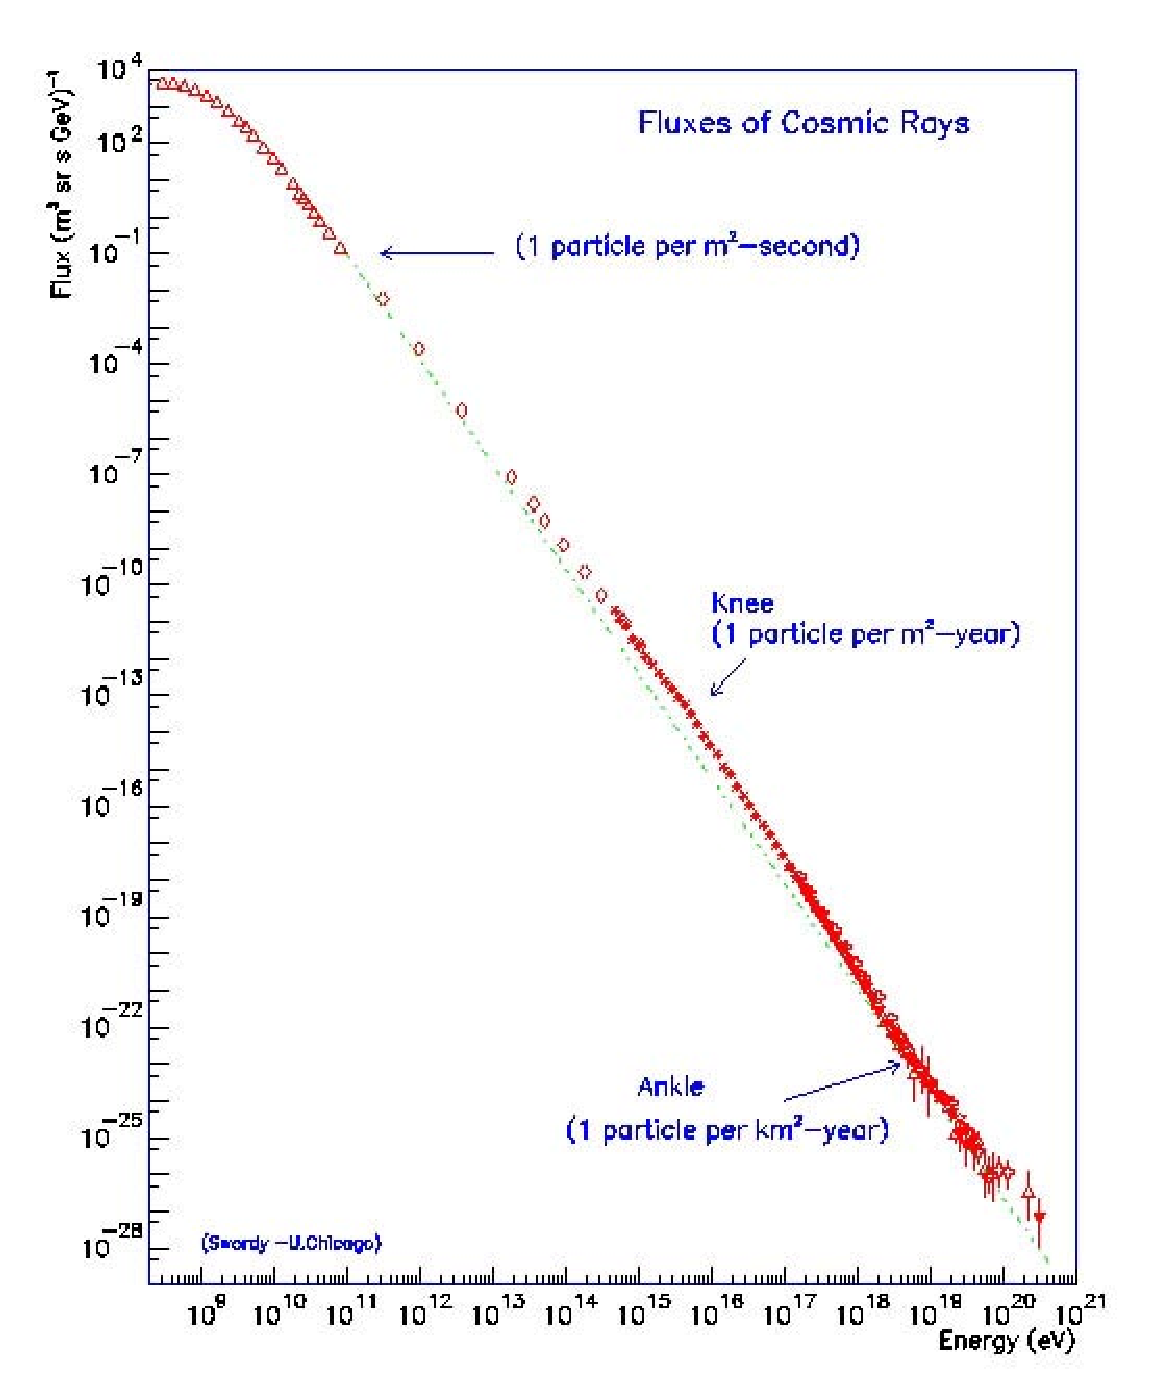
\includegraphics[scale=0.8]{spectrum.eps}
\caption{Measured particle flux of cosmic radiation (the vertical axis) as a function of the energy (horizontal axis). On this double logarithmic scaling we see an almost linear relation, the observed number of particles decreases with increasing energy to the power three. We see two bends in the diagram, named the knee and the ankle, which indicates that different processes influence cosmic radiation. The most right hand side of the graph, the most energetic part, is also shown in more detail in figure~\ref{fig:spectrum_zoom}.}\label{fig:spectrum}
\end{center}\end{figure}

\begin{figure}\begin{center}
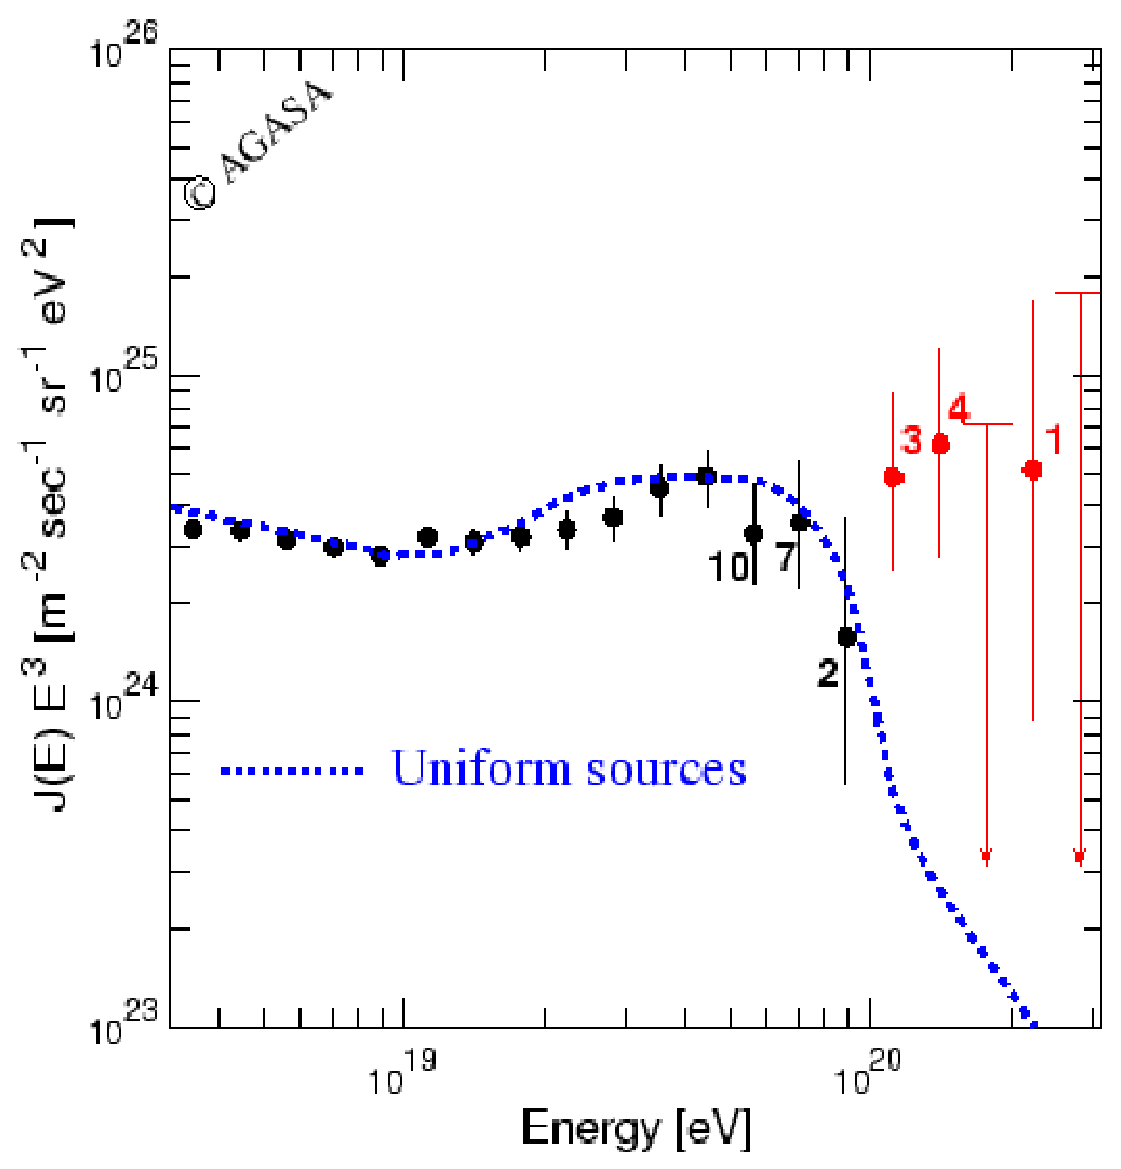
\includegraphics[scale=0.4]{spectrum_zoom.eps}
\caption{Observations from the AGASA-experiment in Japan. The number of observed particles (vertical axis) is scaled with their energy to the power three to obtain this relatively flat curve. The blue dashed line indicates the theoretical expectations, the lines and numbers the actual measurement results with their margins of error.}\label{fig:spectrum_zoom}
\end{center}\end{figure}

\begin{itemize}
\item[-] A large current of protons and other light nuclei with a relatively low energy level, a few MeVs or GeVs per nucleon, come from our Sun. This is the most left hand side of the graph. We call this flow of particle the Solar Winds.\footnote{See the special module `Solar Winds' to read more about them.} The Solar Winds can be a bit unpredictable and can affect electrical systems both on Earth, such as power grids and radio communications, and in space, such as satellites. Therefore they are closely monitored. 
\item[-] Particles with higher energies, up to 10$^{15}$~eV, have their origins mostly inside our galaxy, the Milky Way. These particles do not have enough energy to escape the magnetic field of the Milky Way. Most likely they are produced by shock waves around supernovae.
\item[-] In the region up to 10$^{19}$~eV we see very few particles, less than one particle per square kilometre per year. Even less reach energies of more than 10$^{20}$~eV, or 10 Joule! We do not have a clear answer as to how these particles obtain these tremendous energies. Active galactic nuclei, neutron stars, or supernova remnants are all possibilities, but even those are not able to single handedly give such a large amount of energy to a single particle.
\end{itemize}

\section{Traveling to Earth}
For the low energy particles coming from the Sun the trip to Earth is a short one. The only obstacles in the way are the magnetic fields of the Sun and the Earth. The magnetic field of the Earth does a pretty decent job of keeping most particles out, or at least deflecting them to the poles. This is where the northern and southern lights come from.

The more energetic particles have their origins further away. On their way to Earth they are constantly influenced by different magnetic fields. Even our galaxy as a whole has a weak magnetic field. Weak but large (in area) enough to prevent particles from exiting the galaxy and keep them spinning around in the galaxy until they collide with something.

What about the most energetic particles? Here we run into a different problem. Space is not empty, it is filled with something we call the cosmic microwave background radiation (CMB). This is radiation left behind after the big bang and currently has a temperature of 2.7~K. Per cubic centimetre there are roughly 400 photons with an energy corresponding to a temperature of 2.7~K. When an ultra high energetic proton or other atomic nucleus travels through space it encounters these photons and reacts with them. At energies above 10$^{20}$~eV  there is enough energy to create unstable pions and single protons. These new particles take away a part of the energy of the original nucleus, decreasing its energy.

Reactions with the CMB keep happening until the energy of the cosmic ray falls below 10$^{20}$~eV. Independent of the starting energy, this takes about 100~Mpc, mega parsecs. This effect was first described by Greisen and a little later, but without knowledge of Greisen's work, by Zatsepin and Kuzmin. It is therefore called the GZK-effect.

Because of the GZK-threshold we do not expect the observe any (or hardly any) particles with energies above 10$^{20}$~eV. But the AGASA-experiment did see them, as shown in figure~\ref{fig:spectrum_zoom}. This must mean that there are sources of these extremely energetic particles within 100~Mpc of Earth, but we have yet to find them. The search for these sources is not easy because of the limited number of detected particles. A further complication is the influence of magnetic fields, these deflect and bend the paths taken by the particles. 

\begin{shaded}
\textbf{Exercise \theExercise \stepcounter{Exercise}} : On Earth we measured particles with energies in excess of 10$^{20}$~eV, their origins must lie within 100~Mpc.
\begin{itemize}
\item[-] Convert the unit parsec (pc) into metres and light years.
\item[-] Must the source of these ultra high energetic particles lie within the Milky Way, or can it also be in a different galaxy? Explain your answer.
\end{itemize}\end{shaded}


\end{document}


\begin{shaded}
\textbf{Exercise \theExercise \stepcounter{Exercise}} : \end{shaded}

\footnotemark
\footnotetext{}

\begin{figure}\begin{center}
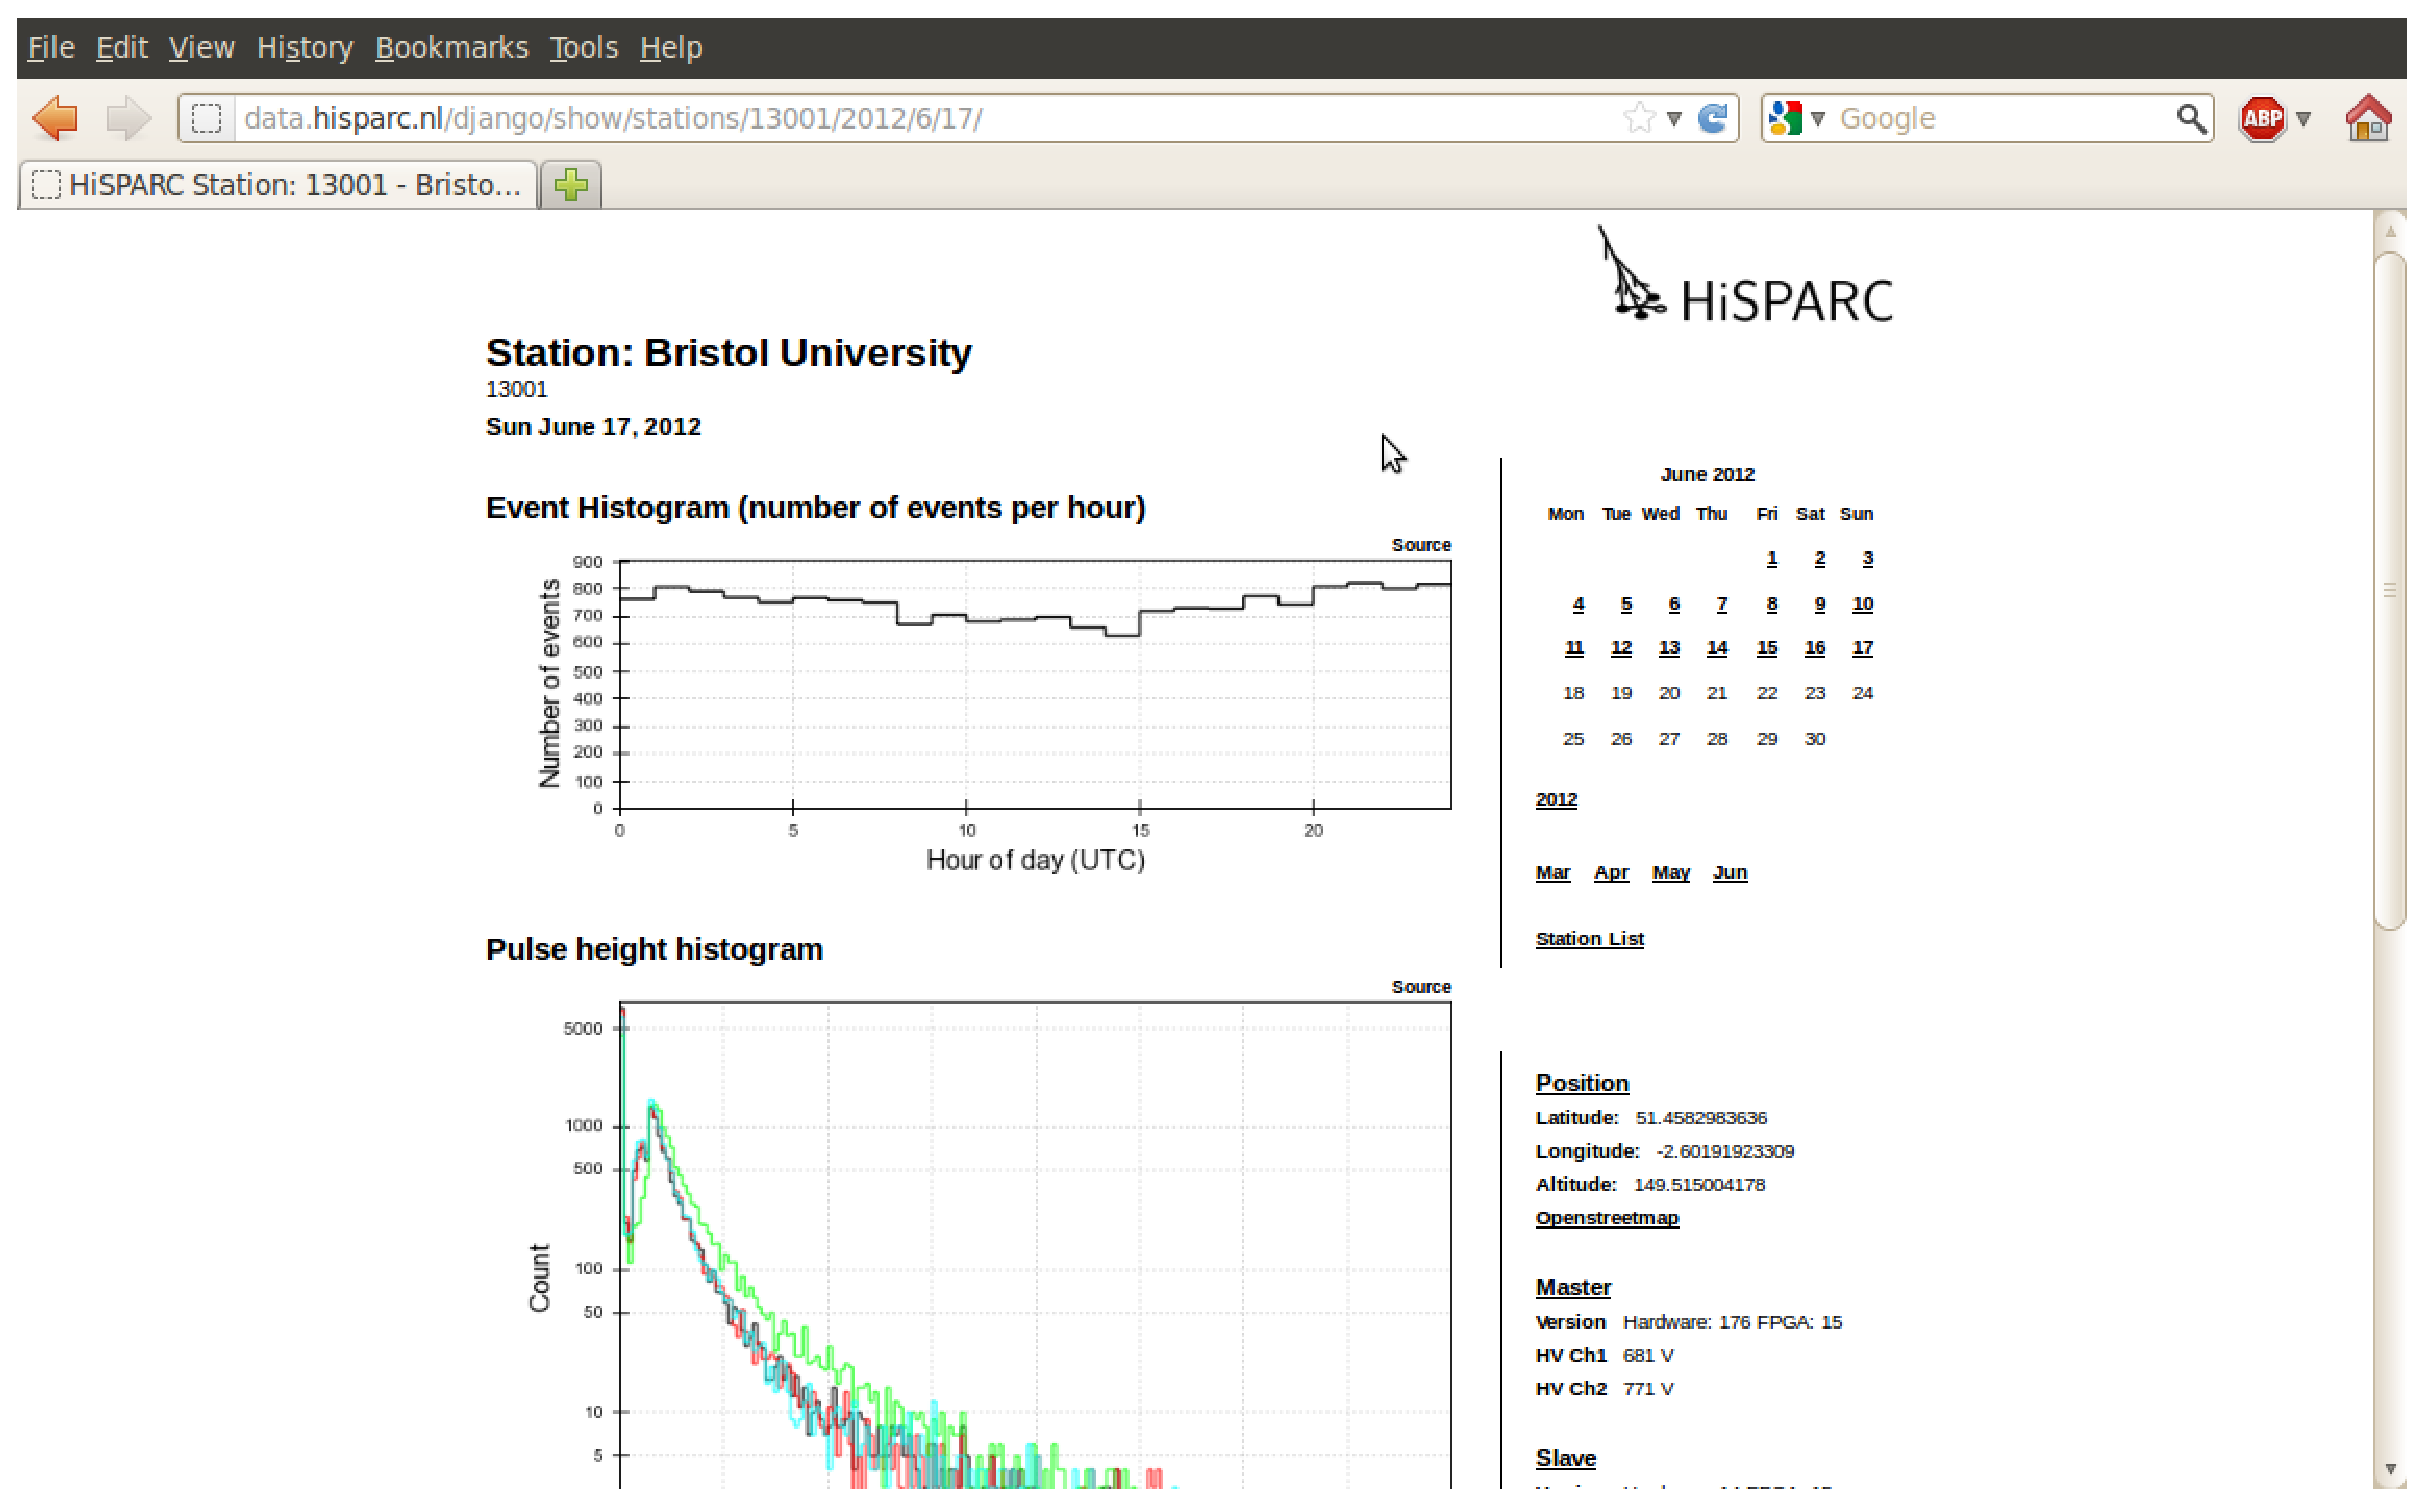
\includegraphics[scale=0.3]{Screenshot_HiSPARC_Station_13001.eps}
\caption{Information available via \protect\url{http://data.hisparc.nl/} .}\label{fig:data_screen}
\end{center}\end{figure}
